\documentclass[10pt]{article}
\usepackage[a4paper,
 tmargin=3cm,
 bmargin=3cm,
 lmargin=2cm,
 rmargin=2cm]{geometry}

% Don't necessarily need all of these, I just copied from my standard LaTeX config
\usepackage{parskip}
\usepackage{graphicx}
\usepackage{wrapfig}
\usepackage[hidelinks]{hyperref}
\usepackage{multirow}
\usepackage{array}
\usepackage{booktabs}
\hbadness 10000 % suppresses underfull hbox errors which are common with marginpar
\usepackage{float}
\usepackage[labelfont=it]{caption}
\captionsetup{belowskip=-0.4cm}
\newcommand{\figref}[1]{\textit{Figure \ref{fig:#1}}}
\usepackage{enumitem}
\usepackage{cmap}
\usepackage[scaled=0.8]{beramono} % This is nice because the tilde isn't at the top of the line.
\usepackage[T1]{fontenc}

\usepackage{tcolorbox}
\tcbuselibrary{listings}
\lstdefinestyle{tcbscript}{language={},
 belowskip=2pt, aboveskip=2pt,
 columns=fullflexible, keepspaces=true,
 breaklines=true, breakatwhitespace=true,
 basicstyle=\ttfamily\small, extendedchars=true, nolol
 }
\newtcblisting{script}[1]{
 title=#1,
 fontupper=\ttfamily,
 fonttitle=\bfseries,
 colframe=blue!60!gray,
 colback=blue!5,
 width=0.95\textwidth,
 center,
 listing only,
 listing style=tcbscript,
 beforeafter skip=0.45cm
}
\newtcblisting{cmdline}{
 fontupper=\ttfamily,
 colframe=white, opacityframe=0, % transparent
 colback=white, opacityback=0, % transparent
 width=0.95\textwidth,
 center,
 listing only,
 listing style=tcbscript,
 beforeafter skip=-0.05cm
}
\newtcolorbox{question}[0]{
 center,
 width=0.95\textwidth,
 colback=red!5!white,
 colframe=red!75!black,
 fonttitle=\bfseries,
 title=Questions,
 beforeafter skip=0.45cm
}

\usepackage{amsmath}
\usepackage{amssymb}
\usepackage[version=4]{mhchem}
\usepackage{chemmacros}
\usepackage{siunitx}
\usepackage{upgreek}

% Bibliography
\usepackage[style=chem-acs,biblabel=dot,subentry]{biblatex}
\addbibresource{sbmmd.bib}
% uncomment if needed

\usepackage{fancyhdr}
 
\pagestyle{fancy}
\fancyhf{}
\rhead{SBM CDT 2020}
\lhead{Practical Computational Chemistry Module}
\cfoot{\thepage}
\begin{document}

\textbf{\LARGE Getting Started with Gromacs -- Day 1}

\section{Background}
For this tutorial we will use the molecular dynamics (MD) package GROMACS (GROningen MAchine for Chemical Simulations). The program was originally developed in the Biophysical Chemistry Department at University of Groningen, and is now maintained by contributors in universities and research centres worldwide. GROMACS is free, open-source (released under the GNU Lesser General Public License (LGPL)), and works natively on a Unix-type system, so if you have any of these operating systems, you can also install it in your computer. Similar to ORCA, GROMACS can only be called using the terminal: there is no graphical interface.

During this tutorial, we will also use the following software:

\begin{itemize}
	 \item Chimera (\url{https://www.cgl.ucsf.edu/chimera/}) to prepare the structure 
	\item VMD (\url{http://www.ks.uiuc.edu/Research/vmd/}) to visualise trajectories
\end{itemize}

The purpose of this tutorial is to give you a ``feeling'' for the typical steps used in practical simulations. Since the time available for this exercise is rather limited, we can only perform very short sample simulations. We will first prepare the crystal structure of a biomolecule and then take a look to the input files necessary for the simulation. Then, we will solvate the structure in water, minimise and equilibrate it, and finally perform a short production simulation. After this, we will run some simple analysis using the tools that are already part of GROMACS.

\textbf{Useful Sources}
\begin{itemize}
	 \item \url{http://www.mdtutorials.com/gmx/}
	\item\ J.\ A.\ Lemkul ``From Proteins to Perturbed Hamiltonians: A Suite of Tutorials for the GROMACS-2018 Molecular Simulation Package'', \url{https://doi.org/10.33011/livecoms.1.1.5068}
    \item M.\ J.\ Abraham, T.\ Murtola, R.\ Schulz, S.\ P\'{a}ll, J.\ C.\ Smith \textit{et al.} GROMACS: High performance molecular simulations through multi-level parallelism from laptops to supercomputers. \textit{SoftwareX} \textbf{2015,} \textit{1--2,} 19--25. \url{https://doi.org/10.1016/j.softx.2015.06.001} 
\end{itemize}

\section{Setting up GROMACS}
In \texttt{arcus-b} there are several version of this software. \begin{figure}[H]
 \centering
 \includegraphics[scale=0.5]{./img/gromacs}
 \caption{GROMACS modules available}
\end{figure}
We will use the following one:
\begin{cmdline}
module load gromacs/2018.6__single
\end{cmdline}

GROMACS is composed of several modules invoked (in this version) with the command \texttt{gmx\_mpi}. For example, the module \texttt{pdb2gmx} is invoked typing: \texttt{gmx\_mpi pdb2gmx}. To get information about any GROMACS module, you can invoke the following command:

\begin{cmdline}
gmx_mpi (module) -h
\end{cmdline}

Other tutorials may use \texttt{gmx} instead of \texttt{gmx\_mpi}. These two are largely equivalent, but depending on how GROMACS was installed on the system one or the other may be appropriate. In our case, we will use \texttt{gmx\_mpi}.

\textbf{Tip of the day}: Organise your input files! We suggest creating a subfolder for each step, placing ``readme'' files in the folders describing what each of them contains.

where \texttt{(module)} is replaced by the actual name of the command you're trying to issue, e.g \texttt{pdb2gmp}, \texttt{grompp}, etc. Information will be printed to the terminal, including available algorithms, options, required file formats, known bugs and limitations, etc. We recommend new users of GROMACS, to invoke the help information for common commands to learn what each of them do. 

Most of the GROMACS jobs can be run directly without a submission script, but for production MD runs it is a good idea to submit the job to the cluster. In order to do this, install a short script using:

\begin{cmdline}
source <(wget -O - https://raw.githubusercontent.com/duartegroup/sbmcc/master/md/qgmxsetup.sh)
\end{cmdline}

From now on, any time you need to run \texttt{gmx\_mpi mdrun -v -deffnm XYZ}, simply replace that command with \texttt{qgmx XYZ}; this will automatically submit the \texttt{mdrun} command to the cluster.

As a ``warm up'', we suggest you complete this tutorial now: \url{http://www.mdtutorials.com/gmx/lysozyme/index.html}. If you are unable to do so, please ask for help, but DO NOT skip steps. Otherwise you will struggle tomorrow. Don't forget to replace any instances of \texttt{gmx} with \texttt{gmx\_mpi}.


\newpage\textbf{\LARGE Getting Started with Gromacs -- Day 2}

\section{Epoxide hydrolase}
In this tutorial we will work with the potato epoxide hydrolase enzyme (StEH1). Epoxide hydrolases (EHs) are enzymes catalysing the hydrolysis of epoxides to yield the corresponding vicinal diol.\autocite{Elfstrom2005} The functions of EHs are diverse, including detoxification through the breakdown of toxic epoxides, catabolism, and cellular signalling. 

\begin{figure}[H]
 \centering
 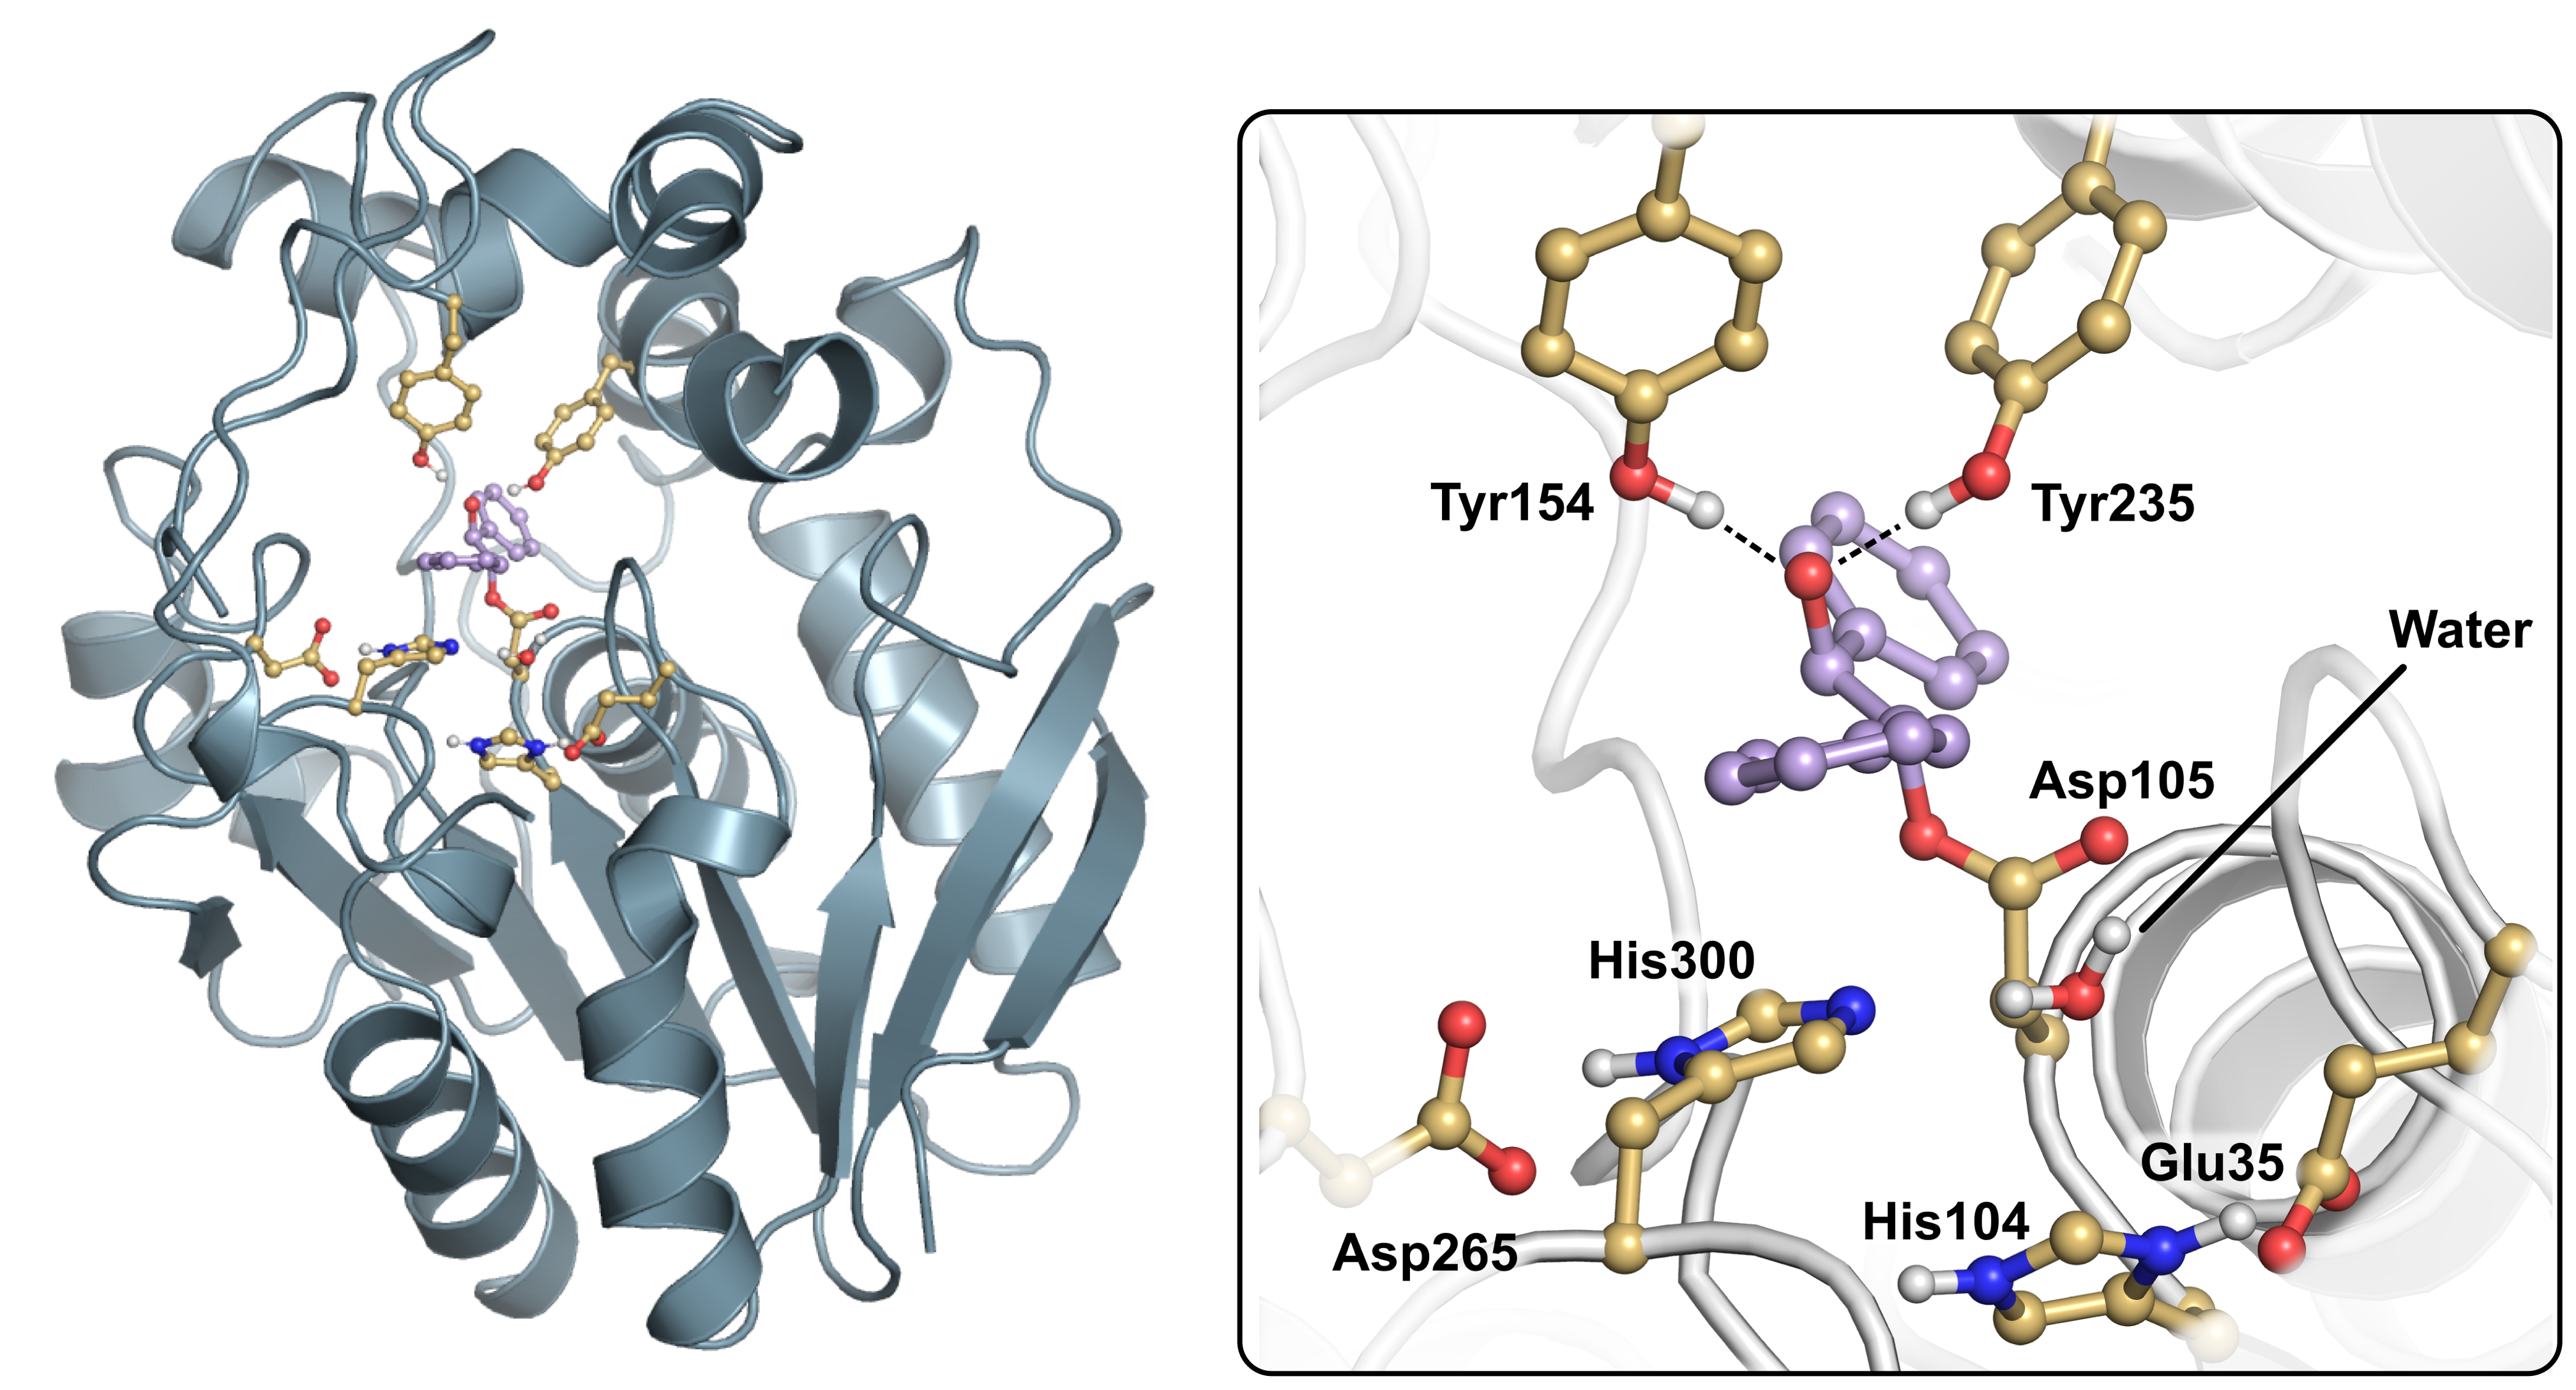
\includegraphics[scale=0.68]{./img/structure}
 \caption{Overall structure of StEH1. Catalytic residues are shown as stick representations.}
\end{figure}

Most EHs belong to the versatile family of $\alpha/\beta$-hydrolase fold enzymes, consisting in a core domain with a central eight-stranded $\beta$-sheet flanked by $\alpha$-helices, as well as a mainly helical domain that forms a lid over the core, so forming the active site. Three residues of the $\alpha/\beta$domain form a catalytic triad (D105, E35, and H300), while two tyrosines of the lid assist in opening the epoxide ring. The distinct catalytic behaviours of mammalian, fungal, and bacterial EHs have been studied extensively.\autocite{Morisseau2005}

\begin{figure}[H]
 \centering
 \includegraphics[scale=0.3]{./img/rxns}
 \caption{Reactions catalysed by StEH1.}
\end{figure}

Here, we will evaluate the quality of the crystal structure. We will also inspect the protein for missing atoms or residues, remove unwanted molecules from our system, and determine the protonation states of ionisable residues (note: in a classical MD simulation, the protonation states are fixed). If our setup had included the substrate, we would also need to parametrise and dock this molecule into the active site. However, for the sake of simplicity, in this tutorial, we will only work with the apo form of the enzyme. 

\section{Structure preparation}

\begin{itemize}
    \item Go to the RCSB website (www.pdb.org) and download the PDB file for the crystal structure (PDB entry 2CJP).\autocite{Mowbray2006} Open the PDB file in a text editor (TextEdit, Notepad). 
    \item Open the PDB structure in Chimera. Familiarise yourself with the program using the online tutorial: \url{http://www.cgl.ucsf.edu/chimera/docs/UsersGuide/tutorials/getting_started.html}
    \item For simplicity, we will remove existing water molecules from the crystal structure. However, active site bound water molecules should be preserved, as they are chemically significant and have high electron densities. To do so, open the 2CJP electron density map (EDS). Select and show all water molecules within a 10~\r{A} radius of the nucleophile D105:
        \begin{cmdline}
            sel :105 zr < 10 & :HOH; display sel
        \end{cmdline}
        Visualise the density of the selection by following this procedure: open \textbf{Tools > Volume Data > Volume Viewer}; open \textbf{Features > Zone} and click the Zone button. 
    \item We will now remove all water molecules outside the 10~\r{A} radius of D105, and also chain B and all non-standard residues. Save the new PDB as \texttt{2cjp\_wat\_10a\_105.pdb}.
    \item Protonation states of ionizable residues (ASP, GLU, LYS, ARG, HIS and rarely CYS, TYR, SER, ASN, GLN) have to be determined before the simulation. To do this, we will calculate \(\mathrm pK_\mathrm{a}\) values of ionizable residues using the H++ server (\url{http://biophysics.cs.vt.edu/}) and assume a pH of 7.0. Acidic residues with a \(\mathrm pK_\mathrm{a}\) below 7.0 and basic residues with a \(\mathrm pK_\mathrm{a}\) above 7.0 will be ionised.

          (Histidine has a \(\mathrm pK_\mathrm{a}\) of about 7.0 in solution, and it is usually necessary to make a visual inspection of the local environment to decide the protonation state. In addition, neutral histidine can exist in two tautomeric forms (HID and HIE).)
\end{itemize}

\begin{question}
    \begin{enumerate}[leftmargin=0.6cm]
        \renewcommand{\labelenumi}{Q\arabic{enumi}.}
        \item Write down the following information in your notebook: crystal resolution, missing residues, non-standard ligands, biological unit, temperature and pH at which the structure was obtained.
        \item With a visualisation program, identify the catalytic residues in your structure.
        \item Are all water molecules in the active site clearly visible in the density map? Can you determine which one is involved in the second step of the reaction?
        \item Obtain the \(\mathrm pK_\mathrm{a}\) and determine the protonation states of ionisable residues. 
    \end{enumerate}
\end{question}

Here we have helped you with Q4:

\begin{center}
    \begin{tabular}{cc|cc}
        \toprule
        Residue & Type & Residue & Type \\
        \midrule
        6       & HIE  & 131     & HIE  \\
        17      & HIE  & 153     & HIE  \\
        31      & HID  & 269     & HIE  \\
        42      & HID  & 278     & HIE  \\
        80      & HIE  & 300     & HIP  \\
        104     & HIE  & 308     & HID  \\
        113     & HID  & 313     & HIE  \\
        \bottomrule
    \end{tabular}
\end{center}


\section{Prepare the topology}

In order to simulate this complex system we will use a simplified representation, where atoms and bonds will be represented by spheres and springs, respectively, and interactions between the atoms will be described using classical mechanics. Therefore the first step will be to decide what set of parameters and form of the mathematical functions we will use to describe the system (the function plus the set of parameters is called a \textit{force field}). This information will be contained in the topology file. 

To create the topology file execute the following steps:

\begin{cmdline}
module load gromacs/2018.6__single
gmx_mpi pdb2gmx -f 2cjp_wat_10a_105.pdb -o eh.gro -water tip3p -ignh -his 
\end{cmdline}

The program will ask you for a force field -- for this tutorial we will use \textbf{Amber99sb} (option ``5''). Then it will ask you to decide on the protonation state for the histidine residues. All aspartates, glutamates, arginines and lysines will be automatically ionised (to change this behaviour, use the flag -inter instead of -his). The program will then write out some information:

\begin{script}{pdb2gmx output}
Generating angles, dihedrals and pairs...
Making cmap torsions...
There are    0 dihedrals,    0 impropers,   15 angles
             0 pairs,       30 bonds and     0 virtual sites
Total mass 270.240 a.m.u.
Total charge 0.000 e
Including chain 1 in system: 5101 atoms 320 residues
Including chain 2 in system: 45 atoms 15 residues
Now there are 5146 atoms and 335 residues
Total mass in system 36363.905 a.m.u.
Total charge in system -5.000 e

Writing coordinate file...
		--------- PLEASE NOTE ------------
You have successfully generated a topology from: 2cjp_wat_10a_105.pdb.
The Amber99sb force field and the tip3p water model are used.
		--------- ETON ESAELP ------------
\end{script}

which indicates that the total charge of the system is \(-5\).

\begin{question} 
    \begin{enumerate}[leftmargin=0.6cm]
        \renewcommand{\labelenumi}{Q\arabic{enumi}.}
        \setcounter{enumi}{4}
        \item Read the help text of \texttt{pdb2gmx -h} and try to find out what the different files it created do, and what options are available for \texttt{pdb2gmx}. 
        \item Open the \texttt{topol.top} file using any available text editor and check what is the information inside it. Take note of the total number of solvent molecules. 
    \end{enumerate}
\end{question}


\section{Adding solvent water around the protein}

Now we will place the enzyme on a box of water molecules. But before adding solvent we have to determine the size and shape of the simulation box should be. Here we will use a cubic box that will extend 1~nm outwards from the molecule.

\begin{cmdline}
gmx_mpi editconf -f eh.gro -o eh_box.gro -c -d 1.0 -bt cubic
gmx_mpi genbox -cp eh_box.gro -cs spc216.gro -o eh_solv.gro -p topol.top
\end{cmdline}

\vspace{-0.3cm}

\begin{question} 
    \begin{enumerate}[leftmargin=0.6cm]
        \renewcommand{\labelenumi}{Q\arabic{enumi}.}
        \setcounter{enumi}{6}
        \item Note that the \texttt{topol.top} file was changed and now contains the water molecules. How many solvent molecules were added? Before you continue it is a good idea to look at this system in VMD. 
    \end{enumerate}
\end{question}


\section{Neutralise your system}

We now must set the total charge of our system to zero and set the ionic concentration to a value similar to the physiologic ionic concentration. For that we will replace water molecules with \ce{Na+} and \ce{Cl-} ions. We will use the \texttt{genion} tool for that. 

This program requires a \texttt{.tpr} file (run input file) and we haven't generated one so far. We need to create it. For that we will use another tool called \texttt{grompp} (GROMACS pre-processor). This tool allows creating the run input file from a topology; coordinate file, and a simulation parameter input file. 

This file contains all the parameters to run the simulation, such as type of run, number of steps, electrostatics and van der Waals options. We will use this file for the energy minimisation on the next step. 

Run the \texttt{grompp} tool and then run \texttt{genion}:
\begin{cmdline}
gmx grompp -f min.mdp -c eh_solv.gro -p topol.top -o ions.tpr
gmx_mpi genion -s ions.tpr -o eh_neutral.gro -p topol.top -neutral -conc 0.154 
\end{cmdline}

When prompted, choose group 13 ``SOL'' for embedding ions. You do not want to replace parts of your protein with ions.

\section{Energy minimisation}
Before we can begin dynamics, we must ensure that the system has no steric clashes or inappropriate geometry that could lead to large forces and structure distortion. To remove this forces the structure is relaxed through a process called energy minimisation. The aim is not to reach any local energy minimum, but only remove clashes so e.g. 1000 steps of steepest descent algorithm works well for minimisation. The settings for this calculation are defined in a parameter file called \texttt{min.mdp}:
 
With these parameters we are requesting the steepest descent algorithm for energy minimisation with a total of 2000 steps. For the calculation of electrostatics interactions we use the Particle-Mesh Ewald (PME) method and for the van der Waals a cut-off method, with a cutoff of 10~\r{A}.

We generate the run input file for the energy minimisation using \texttt{grompp}:

\begin{cmdline}
gmx_mpi grompp -f mim.mdp -c eh_neutral.gro -p topol.top -o min.tpr
gmx_mpi mdrun -v -deffnm min
\end{cmdline}

You will generate a new structure file containing the new coordinates after the energy minimisation (\texttt{min.gro}), a file with the energies (\texttt{min.edr}), and a log file (\texttt{min.log}). 

To check if the minimisation was successful we should make sure the potential energy is negative and that the maximum force, Fmax, the target for which was set in \texttt{minim.mdp} - ``emtol = 1000.0'' is fulfilled (check it at the end of the log file). To see how the potential energy of the system varies during the minimisation use the following function:

\begin{cmdline}
gmx_mpi energy -f min.edr -o potential.xvg
\end{cmdline}

Choose option 12. Then plot the file \texttt{potential.xvg} with \texttt{xmgrace} or any other graphing software:

\begin{cmdline}
xmgrace potential.xvg
\end{cmdline}

\section{Equilibration of waters around the protein at constant volume}

Now we have a reasonable starting structure. However, in order to perform dynamics on the system we need to equilibrate the solvent and ions around the protein. This relaxation should take around 1~ns; however, due to time constraints we will only use 100~ps (50000 steps). After we arrive at the correct temperature (based on kinetic energies), we will apply pressure to the system until it reaches the proper density. The settings used are:

\begin{script}{nvt.mdp}
title                   = OPLS Lysozyme NVT equilibration 
define                  = -DPOSRES  ; position restrain the protein
; Run parameters
integrator              = md        ; leap-frog integrator
nsteps                  = 50000     ; 2 * 50000 = 100 ps
dt                      = 0.002     ; 2 fs
; Output control
nstxout                 = 500       ; save coordinates every 1.0 ps
nstvout                 = 500       ; save velocities every 1.0 ps
nstenergy               = 500       ; save energies every 1.0 ps
nstlog                  = 500       ; update log file every 1.0 ps
; Bond parameters
continuation            = no        ; first dynamics run
constraint_algorithm    = lincs     ; holonomic constraints 
constraints             = h-bonds   ; bonds involving H are constrained
lincs_iter              = 1         ; accuracy of LINCS
lincs_order             = 4         ; also related to accuracy
; Nonbonded settings 
cutoff-scheme           = Verlet    ; Buffered neighbor searching
ns_type                 = grid      ; search neighboring grid cells
nstlist                 = 10        ; 20 fs, largely irrelevant with Verlet
rcoulomb                = 1.0       ; short-range electrostatic cutoff (in nm)
rvdw                    = 1.0       ; short-range van der Waals cutoff (in nm)
DispCorr                = EnerPres  ; account for cut-off vdW scheme
; Electrostatics
coulombtype             = PME       ; Particle Mesh Ewald for long-range electrostatics
pme_order               = 4         ; cubic interpolation
fourierspacing          = 0.16      ; grid spacing for FFT
; Temperature coupling is on
tcoupl                  = V-rescale             ; modified Berendsen thermostat
tc-grps                 = Protein Non-Protein   ; two coupling groups - more accurate
tau_t                   = 0.1     0.1           ; time constant, in ps
ref_t                   = 300     300           ; reference temperature, one for each group, in K
; Pressure coupling is off
pcoupl                  = no        ; no pressure coupling in NVT
; Periodic boundary conditions
pbc                     = xyz       ; 3-D PBC
; Velocity generation
gen_vel                 = yes       ; assign velocities from Maxwell distribution
gen_temp                = 300       ; temperature for Maxwell distribution
gen_seed                = -1        ; generate a random seed
\end{script}

In this case, we are performing molecular dynamics with an integration time step of 2~fs in a canonical (NVT) ensemble. We are restraining the position of the protein heavy atoms to their initial positions using the \texttt{posre.itp} file generated on step 2. The temperature is controlled using of v-rescale algorithm. The LINCS (Linear Constraint Solver) algorithm is used to constrain bond distances, allowing us to use a larger time step. 

Proceed as before:

\begin{cmdline}
gmx_mpi grompp -f pr1.mdp -c min.gro -p topol.top -o pr1.tpr
\end{cmdline}

Run using the batch system with the following script:

You will generate a new structure file (\texttt{pr1.gro}) containing the new coordinates, a file with the energies (\texttt{pr1.edr}), a log file (\texttt{pr1.log}), and a trajectory file (\texttt{pr1.trr}). You can view the trajectory using the VMD program. Open first the \texttt{.gro} file and then the trajectory file above it. 

Analyze the temperature progression using energy:
\begin{cmdline}
gmx_mpi energy -f pr1.edr 
\end{cmdline}

Type ``15 0'' at the prompt to select the temperature of the system and exit. The resulting plot can be seen using \texttt{xmgrace}

\begin{question}
    \begin{enumerate}[leftmargin=0.6cm]
        \renewcommand{\labelenumi}{Q\arabic{enumi}.}
        \setcounter{enumi}{7}
        \item Has the energy and temperature converged? How could you confirm that your thermostat is correctly implemented?
    \end{enumerate}
\end{question}


\section{Equilibration of the water molecules at constant pressure}

The previous step, NVT equilibration, stabilised the temperature of the system. Prior to data collection, we must also stabilise the pressure (and thus also the density) of the system. Equilibration of pressure is conducted under an NPT ensemble, wherein the Number of particles, Pressure, and Temperature are all constant. The ensemble is also called the ``isothermal-isobaric'' ensemble, and most closely resembles experimental conditions.

\begin{question}
    \begin{enumerate}[leftmargin=0.6cm]
        \renewcommand{\labelenumi}{Q\arabic{enumi}.}
        \setcounter{enumi}{8}
        \item The \texttt{.mdp} file used for a 100~ps NPT equilibration is similar to the previous one. Identify the differences; why has \texttt{gen\_vel} changed from yes to no?
    \end{enumerate}
\end{question}

Use the same script as before, only changing pr1 to pr2:

\begin{cmdline}
gmx_mpi grompp -f pr2.mdp -c pr1.gro -p topol.top -o pr2.tpr
\end{cmdline}

Let's analyze the pressure progression, again using energy:
\begin{cmdline}
gmx_mpi energy -f pr2.edr -o pressure.xvg
\end{cmdline}

Type ``16 0'' at the prompt to select the pressure of the system and exit. 


\section{Production MD}
Finally,  we will run the production simulation for 1~ns (1000000 steps) with no restraints in an NPT ensemble. We will save the trajectory coordinates every 500 steps. Create the \texttt{md.mdp} file with the following information:
 
\begin{cmdline}
gmx_mpi grompp -f md.mdp -c pr2.gro -p topol.top -o md.tpr
\end{cmdline}

and run it with:

\begin{cmdline}
qgmx md.tpr
\end{cmdline}

Remember that such a simulation time is too short to obtain any meaningful result. In practice, one would also need to run many replicas, i.e.\ calculations with the same structures and different initial random velocities. Ideally, with current computer power, you can run 100~ns per day and multiple trajectories (so your total simulation time is larger!). Sometimes you can have simulations that are stable during 400~ns, and then the main changes take place after 500~ns. It all depends on what the relevant timescale for the behaviour at hand is.

\section{Analysis}
We will now analyse the trajectory. Let's start by calculating the root-mean-square deviation of the backbone atoms:
\begin{cmdline}
gmx_mpi rms -s md.tpr -f md.xtc -o rmsd.xvg
\end{cmdline}

Plot the graph using \texttt{xmgrace} or \text{gnuplot} or any other plotting software. We also analyse the hydrogen bonds (H bonds). For this, open your trajectory (\texttt{.xtc}) and \texttt{.gro} file, with vmd. (If vmd crashes with a segfault, it's probably because you do not have enough RAM; a workaround is to increase the Stride to 10 (or 100) when opening the trajectory.)

Alternatively you can use the \texttt{hbond} program. 
\begin{cmdline}
gmx_mpi hbond -s md.tpr -f md.xtc -hbn
\end{cmdline}


If you want to follow a particular H bond, you need to create an index file with the program \texttt{make\_ndx}:

\begin{cmdline}
gmx_mpi make_ndx -f md.gro -n index.ndx -o index.ndx
\end{cmdline}

and select the pair of atoms you want to follow. We suggest to monitor hydrogen bonds for the following residues: H104, E35, D105, and H300. 

\begin{question}
    \begin{enumerate}[leftmargin=0.8cm]
        \renewcommand{\labelenumi}{Q\arabic{enumi}.}
        \setcounter{enumi}{9}
        \item What are the most flexible parts of the protein?
        \item How could you determine if the protein is stable during the simulation time?
    \end{enumerate}
\end{question}

\printbibliography

\end{document}
